\documentclass{acm_proc_article-sp}

\title{3D Printing in Lock Picking}

% NOTE FROM SIGITE WEBSITE: "All other submissions (papers, lightning talks, and posters) should be anonymous, with all author information removed."
% \numberofauthors{3}
% \author{
% % First author
% \alignauthor Byron Doyle\\
%     \affaddr{Brigham Young University}\\
%     \affaddr{School of Technology}\\
%     \affaddr{265 Crabtree Building}\\
%     \affaddr{Provo, UT 84602}\\
%     \email{byrondoyle@gmail.com}
% % Second author
% \alignauthor Colby Goettel\\
%     \affaddr{Brigham Young University}\\
%     \affaddr{School of Technology}\\
%     \affaddr{265 Crabtree Building}\\
%     \affaddr{Provo, UT 84602}\\
%     \email{colby.goettel@gmail.com}
% % Third author
% \alignauthor Dale Rowe\\
%     \affaddr{Brigham Young University}\\
%     \affaddr{School of Technology}\\
%     \affaddr{265 Crabtree Building}\\
%     \affaddr{Provo, UT 84602}\\
%     \email{dale\_rowe@byu.edu}
% }

% Force footnotes to stay on the same page and not bleed over. Long footnotes should be placed in the appendix.
\interfootnotelinepenalty=10000

\begin{document}
\maketitle

\begin{abstract}
    Physical security analysts have always sought to overcome challenges in security infrastructure using novel approaches and new technology. One of these challenges is preset, mechanical lock mechanisms.\footnote{A locking mechanism that is opened by predefined key.} 3D printing technology provides a valuable tool for those interested in attacking or bypassing high-security locks. This technology can allow such practitioners to create key blanks or replicas from key data such as physical key measurements or photographic evidence.
\end{abstract}

\category{K.6.5}{Management of Computing and Information Systems}{Security and Protection}[Unauthorized access] 
\category{I.4.9}{Image processing and computer vision}{Applications}
\category{J.6}{Computer-Aided Engineering}{Computer-aided manufacturing}[CAM]

\terms{Security}
\keywords{Physical security, penetration testing, physical lock, 3D printing, computer aided design}

\section{Introduction}
Preset, mechanical locks are generally vulnerable to a variety of attacks, but due to the enormity of designs and technologies in the world today, each lock typically requires a different technique to exploit or bypass. For example, simple pin and wafer locks can be picked with moderate skill, but more complicated locks with sidebar mechanisms make picking impractical without specialized tools and a high degree of skill. These factors and more must be recognized by information security practitioners because physical access controls for sensitive infrastructure are just as important as logical access controls. No amount of digital security is enough if attackers can bypass the physical security and gain direct access to hardware.

Impressioning is a common lock picking technique that allows an attacker to create a copy of the key for the target lock. However, it requires a decent amount of skill and key blanks specific to the target lock type. Another option is to have the key copied, but there are countermeasures in place to make this difficult. These countermeasures include controlling the key blanks and cutting facilities for high-security locks. Additionally, it is inherently difficult to obtain the bitting\footnote{A code that defines the key cuts that will properly open the target lock.} of the original key.

3D printing can make all of these attacks more effective, increasing the risk that high-security locks may be circumvented. To understand how these manufacturing techniques can be used, a few methods of 3D printing will first be discussed, including their benefits and drawbacks. Next, some popular attacks on preset, mechanical lock systems will be examined. Finally, the two approaches will be combined to understand how 3D printing technology can enhance lock picking high-security locks.

\section{3D Printing Techniques}
3D printing, a form of rapid manufacturing, is a broad field with various methods of producing products in a variety of materials. Each of these techniques has pros and cons for the penetration of physical security systems. Notable techniques include are fused filament modeling, stereo lithography, and direct metal laser sintering.

\subsection{Fused Filament Fabrication}
Fused filament fabrication (FFF)\footnote{Also called fused deposition modeling (FDM).} is one of the commonest and cheapest 3D printing techniques. Relatively high quality models are built out of various types of plastic by a machine that lays down traces of material in patterns, building up layers in the $z$-axis \cite{VALAVAARA}.

Fused filament fabrication is one of the largest areas of new material development due to the relatively high adoption rate in the consumer market. Typically, prints are produced in either ABS\footnote{Acrylonitrile butadiene styrene, a common thermoplastic used in the manufacturing of cheap, mass-produced parts.} or PLA,\footnote{Polylactic acid, a biodegradable thermoplastic made out of various renewable resources such as corn starch and sugar cane.} but many materials can be used for a given application. FFF-manufactured parts have different properties depending on the material they are made from, so it is important to choose the right material for the application. ABS plastic offers a good balance of hardness and flexibility, both of which are important when producing parts like thin key blanks. PLA is more rigid, but also more likely to snap rather than bend.

This method is particularly useful because of its availability: a 3D printer with the accuracy required to produce basic key blanks can be purchased for under \$500. However, if that option is not available, there are many online services that offer high-quality and fairly-priced prints using this method.

Of particular interest to this topic may be nylon. Nylon materials specific to 3D printing are designed to offer a wide range of characteristics depending on the temperature they are printed at; this builds off the innate properties of the material. Warmer temperatures will yield an extremely strong bond and hard part. Cooler temperatures result in a more flexible part with weaker bonds. In addition, nylon is extremely abrasion-resistant which is important for working in locks without leaving behind plastic shavings.

\subsection{Stereolithography}
Stereolithography (SLA) is the original 3D printing process, first patented in 1984. This process is characterized by the transformation of a liquid photopolymer into a solid by a laser or other curing light element \cite{HULL}. In most situations, this process produces some of the highest-resolution models available.

The cost of stereolithography equipment is generally more than FFF equipment. Consumer-level printers range from \$2000 to \$3000. These machines provide a build volume\footnote{The total volume in which a 3D printer can construct a part; the limiting factor in the size of any one print job.} large enough for keys while still maintaining a relatively low cost. Online 3D printing services can provide larger, higher quality prints as well which could be valuable when mass-producing parts.

High resolution is paramount in the design of complex keys and key blanks. The higher resolution and bonding method of SLA can produce stronger models, though strength varies with the type of material used. This printing process necessitates the addition of support sprues to the model; these must be taken into account when designing precision-driven projects such as keys, as the connection points between the part and the sprues leave small bits of material that must be carefully filed away.

Materials for SLA machines are more limited in variety than their FFF counterparts. Photopolymers for SLA printing generally resemble ABS after being cured. Unlike thermoplastics, however, photopolymers will continue to cure as long as they are exposed to ultraviolet light. Depending on the material used, parts made with photopolymer liquids can become brittle over time as they over-cure through exposure. Materials research continues to mitigate this effect, but because of the material development cost, the relatively low demand, and the relatively high production cost, liquid photopolymer materials are often quite costly.

\subsection{Direct Metal Laser Sintering}
Direct metal laser sintering (DMLS) is a manufacturing method that creates solid metal parts by exposing and bonding fine metal powders with a high-power laser \cite{DAS}. This process differs from the others in that it can create metal parts which rival or exceed the strength of cast parts and, in some cases, even forged parts. Parts produced with this process are extremely accurate and typically have a very smooth finish.

The benefits of this process may be less obvious as DMLS equipment is not available directly to consumers. However, DMLS is now a common format available through online 3D printing services, making it especially useful when custom one-off tools are required or when a controlled key blank distribution system (such as with many high-security locks) must be circumvented.

Since DMLS parts are typically expensive, it is usually better to use another form of 3D printing to produce early prototypes. Only after the design is finalized should the part design be sent off for DMLS manufacturing. DMLS should be thought of as an option only for high fidelity, high strength prototypes and finished products.

Many different metals can be used with DMLS, the material only needs to have stable thermal properties over its melting point. As the technology advances, more metals are made available for manufacturing. Titanium is a very popular material as it is light, strong, and corrosion resistant. Steel and brass are also popular, but are more often offered online as casts from a 3D printed wax or sand model. These parts typically offer good strength, but their surface finishes are not as accurate.

\section{Popular Attacks on Preset Mechanical Lock Systems}
\subsection{Lock Picking}
Lock picking is the most famous attack on preset mechanical lock systems, though not always the most effective. A small torque is applied to the keyway of the lock or cylinder of the lock, and the pins of the lock are pushed up slowly until the pin tumblers sitting on top of the pins engage the shear line between the lock cylinder and the lock body \cite{TOOOL1}.

\begin{figure}[htb]
    \centering
    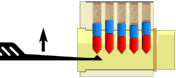
\includegraphics{lockpicking}
    \caption{Side view of the lock picking process \cite{TOOOL1}.}
    \label{lockpicking}
\end{figure}

This attack can also be used, with the appropriate tools, on wafer locks, tube locks, and others. Wafer locks are opened in much the same way as pin tumbler locks, but with one key difference: the shear line is wide and the wafers all engage a single large slot. This allows for a large amount of play in the workings of the lock, making picking much easier. Tube locks are easier to pick for a different reason: they only require a special tool, conveniently called a ``tube lock pick.'' The tool is engaged with the lock, and torque is applied on and off while the tool is gently pressed down. The binding of the pins against the shear line of the lock impression the bitting of the tube lock into the lock pick.

Raking is performed by dragging a tool lightly across the bottom of the pins while applying light torque to the lock cylinder. As the tool bumps against the pins, they rebound against the pin tumblers which should rise above the shear line and set. This can be done very quickly to open simple locks. This technique varies greatly depending on the tools used, the target lock, and the attacker's preferences and skill. Many different pick shapes can be used for raking, but typically half-diamond, hook, and snake shapes are preferred. The target lock's geometry affects how raking is performed and if it is useful. This is typically a function of the pick shape in contrast to the keyway\footnote{The cut in the lock cylinder through which the body of the key passes.} shape.

Scrubbing is a variation of raking: instead of dragging a tool across the pins, a wide, flat tool is used to push groups of pins up and down in a tooth brushing motion. In this way the attacker is effectively attempting to pick multiple pins at once. This technique is extremely useful when raking fails because of restrictive keyway shapes or when the target lock's pins are very close together. Scrubbing may also be preferred if the spring tension on the pins is high~--- a common trait of padlocks and other outdoor locks. Scrubbing is sometimes used instead of raking because of preference; however, both raking and scrubbing are equally useful.

Bumping is a variation of the raking technique using a specialized key blank, cut just past the deepest pin depth on all pins with ridges in-between. This tool is called a bump key, or 999 key.\footnote{So-called because the key is cut to a modified all-nines bitting} The bumping technique is performed by pulling the bump key slightly out of the lock, applying light torque, and then lightly bumping the key with a wooden hammer or other apparatus in order to strike all the pins at once. This forces all the pin tumblers above the shear line at once, opening the lock.

Raking and scrubbing generally fall together as the two techniques experienced lock pickers use to quickly open easy-to-bypass locks. These techniques are most useful, however, when combined with skillful single-pin picking: problematic pins can be set, and then raking or scrubbing can be used to set the rest. Bumping expands on raking by using specialized key blanks made specifically to set all the pins in the target lock at once. With the proper tools and some practice, lock bumping can open hard-to-pick locks.

\subsection{Impressioning}
Physical decoding of a target lock is performed through impressioning. A specially-prepared key blank is used to make a copy of the key for the target lock. This key reflects the lock's bitting. The blank is placed in the lock, torque is applied, and the key is moved up and down against the pins; any pin at the improper height will be bound against the sides of the lock body and cylinder. This binding friction slightly marks the pins on the blank. The key is then removed from the lock, inspected for marks, and cut with a file where they are found. Cuts are made one bit-depth at a time, and the process is repeated. This can be done for all pins in the lock at once under normal circumstances. If the attack is successful, the attacker will end up with a working key. The only caveat is that the attacker must apply the proper torque and force on the pins: too little torque or too much force and the pins will slip, causing missed bittings; too much torque or too little force and the pins will bind in the wrong places, causing false positives. Either of these mistakes will damage the target lock.

Attackers should use caution with this technique because improper use can lead to positive indications of an attack on the lock. In some cases, locks may degrade quickly and seize or bind because many shear forces are being applied to the inner bearing surfaces of the lock in an unusual manner. If discretion is required, care should also be taken to thoroughly clean the filed blank before re-inserting it into the target lock. Leaving loose metal shavings inside the lock is a fairly obvious giveaway, as filings from regular use typically differ from those resulting from filing a key blank. The permanence of impressioning is also very useful for quiet attacks: an attacker can slowly impression a lock over a space of days or weeks by taking one sample at a time and then leaving, only to return later.

\subsection{Copying}
The biggest difficulty when making a copy of a key is exactly duplicating the key's bitting. This can be done via certain lock picking techniques, such as using a tube lock pick, impressioning, using a pin lock decoder, or by gaining physical access to the key in order to take measurements or a mold. This is difficult because all of these techniques can be quite intrusive.

One technique for decoding keys from a distance was developed by Laxton, Wang, and Savage \cite{LAXTON}. It involves taking photos of a key from a distance and then using computer vision algorithms to decode the bitting. This proved equally successful up close and at a distance using long-focus lenses. This technique removes the attacker from the immediate vicinity of the key owner and is much less intrusive. More powerful optics could be used to not only capture key information without the risk of notifying the target, but also to keep the attacker completely out of view. This entirely obviates the security of sole key ownership of common locks because key copying facilities are widely available. Key blanks are freely available and copies can often be manufactured without providing the original key.

Copies of keys from impressioning are also extremely useful for providing the bitting for a lock. Because they must open the lock for the attack to be successful, the original impressioned key can be regarded as the lock's decoded bitting. This can then be used to create copies of the target key that appear genuine in order to facilitate a more successful attack. This is especially true of keys for high-security locks; typically, high-security blanks are only provided by the lock manufacturer, resulting in every key looking similar. Depending on the manufacturing techniques used, impressioned keys can be copied with the minutest details intact, producing incredibly realistic functional facsimiles.

In order to fool people, attackers need to consider that an entirely new key is being produced during the copying process, but probably should not look brand new. High-security-keys, however, have more exploitable features so care must be taken when making copies in order to replicate not only the working parts of the key, but the aesthetic portions as well. If photos of a target key are taken, an exact replica can be made: the replica can be weathered to match the original, serial numbers can be matched, logos can be copied. These features all add up making a key that has history in a social context; it can be used in social engineering attacks as well as to open doors.

\section{Augmenting Attacks with 3D Printing}
The attacks described above can all be augmented by 3D printing in a variety of ways, depending on the printing processes and materials used. One notable use of the technology is the ease of making specialized tooling to attack high-security locks such as the ASSA Twin Series. These locks have a coded sidebar preventing the lock from turning independently of the top pins. Both blanks, spare parts, and discarded cylinders are carefully controlled.

\begin{figure}[htb]
    \centering
    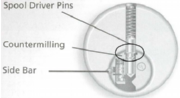
\includegraphics{spool}
    \caption{Internal diagram of ASSA Twin Series lock \cite{TOOOL2}.}
    \label{spool}
\end{figure}

\subsection{Lock picking}
3D printing allows the cheap manufacturing of specialized tools for lock picking. To facilitate a lock picking attack against a Twin Series lock, a special torsion wrench, with the correct sidebar bitting built in, could be printed. The top bitting may be unknown as it is unique to each lock, but sidebar bittings are set by region. Thus any sample key from the target site may lead to a more complete exploitation of the security system.

In the case of torsion wrenches or other force-applying tools, a stronger-bonding polymer process (like SLA) or a metal printing process (like DMLS) could be more useful than the cheaper fused filament fabrication process found in consumer-level 3D printers. The designer must decide how much torque is required for the application and how that torque will be applied through the tool. The designer can then choose a manufacturing process with this information.

For permanent or reusable tool manufacturing it is useful to design and implement a prototype version in a plastic format because it is cheaper and more readily producible. These prototypes can then be evaluated and iterated upon as needed. To provide longevity and strength in the tool, a final version can be made using a metal printing process. This might be especially useful for creating specialized tools that are not specific to a certain lock bitting, but are specific to an application; for example, a bypass tool for a lock with a common vulnerability found during the picking process.

Bump key manufacturing benefits greatly from this process as well, especially in the case of high-security locks. Bump keys are normally made out of stock key blanks; however, manufacturer controls limit this process in the case of high-security locks. To circumvent this, a complete bump key can be designed, tested, and then printed in metal. Since bump keys are only specific to the type of lock, and not the bitting, such tools are still useful when the target lock has been exploited.

\subsection{Impressioning}
The applications of 3D printing for impressioning are a natural extension of the applications in lock picking. ASSA is deliberately protective over key blank distribution and key cutting for their locks, as it increases security. However, with 3D printing, a blank can be manufactured for the lock based on any cut key sample and rough specifications of the lock; both of these are easily acquired via proper reconnaissance, or photography and computer vision.

In practice, creating blanks for high-security locks using low-cost, 3D printing tools is very easy. Figure~\ref{model} shows a 3D model created from physical measurements taken from samples of ASSA Twin Series keys; this model has been used to successfully print key blanks on a consumer-level FFF 3D printer. These key blanks were printed in PLA, a stiff but malleable plastic. Impressioning with plastic blanks manufactured this way should work quite well if used in conjunction with a torsion wrench to apply torque to the lock after the sidebar bitting is modeled into the blank.

\begin{figure}[htb]
    \centering
    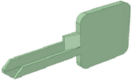
\includegraphics{model}
    \caption{3D model of an ASSA Twin Series key blank.}
    \label{model}
\end{figure}

In some high-security locks it may be possible to impression the sidebar when the top-bitting is known but the sidebar bitting is not (for example, if a picture of the back of an original key is used to decode the lock). In this case, a key with a coded top bitting and a blank sidebar would be printed, and impressioning would be performed as usual. Depending on the lock's sidebar mechanism this may not work~--- the ASSA Twin Series uses a sidebar mechanism where this is not possible. Other locks with sidebar mechanisms, such as Medeco high-security locks, may have more success.

If correctly designed, blanks can be used repeatedly for the same type of lock without care for specific fitment within the same lock model. Once such a design is achieved for a high-security lock, the blank can be publicly released. Public release of blank models removes the security advantages of limiting blank distribution. Easy access to 3D printing facilities ensures that attackers can easily access blanks. Blank distribution limitations may actually become a liability as the availability of printed blanks could exceed the availability of legitimate ones, putting control of distribution firmly out of the hands of the manufacturer.

\subsection{Copying}
After a lock or its key is decoded by impressioning, computer vision, or other means, a true copy of the key can be made via 3D printing as well. At this point, a metal printing process should be used if the goal is to have a permanent key; otherwise, a copy could be printed and torque applied with a torsion wrench to open the lock. In both cases this implies a persistent threat to the preset system: even if the copy is recovered by the affected organization, another can be made without need for special tooling or blanks, just a CAD file.

The usefulness of 3D printing in key copying is perhaps the most obvious, but warrants extra consideration. When fine detail is needed, an exact duplicate can be made, down to the numbering, logos, and simulated wear, if properly modeled. During a penetration test this may be extremely useful as a social element: in addition to the key working, it can also be shown to personnel as proof that the attacker is supposed to be there. For example, a copy of a key can be made, worn down, and then taken to a facilities office under the pretense that it no longer works. The key can then be traded for a new, properly serialized key from the organization~--- the forged key is no longer in circulation, the attacker has a real key, and the original key will stay in circulation until it is turned in or audited.

\section{Conclusion}
The capabilities of 3D printing technology have posed a persistent threat to organizations' physical infrastructures for quite a while. This is done by clever manipulation of lock picking, impressioning, copying, and other means. Essentially, the supply chain control paradigm for high-security physical locks will no longer stop a determined attacker from gaining physical access to what those locks are protecting. For this reason, new security models need to be put in place for physical security, and lock manufacturers need to stop relying on outdated supply chain control and innovate.

The methods presented here can be used to create custom tools to address even the most obscure physical security platforms. A clever attacker no longer has to worry about security through obscurity in the physical space and can fill his toolbox with items meant specifically to address the physical security weaknesses of a targeted organization. These tools afford the same flexibility to the attacker in the physical space as he already has in the digital space. A physical key can be copied and used without notifying the original owner, compromised in the same manner a digital key would. A physical system can be reverse-engineered without leaving evidence behind, quietly probing a secure system over a long period of time. Security access controls can be bypassed entirely as evidence for social attacks appears out of only collected data.

3D printing is advanced enough that complete copies of legitimate keys can be made, akin to copying organizational IDs or badges. These keys can be used in social attacks, as well as to open doors and gain access to physical spaces. For security professionals, this means looking at physical security threats in a new way, as attackers are not necessarily impeded by physical access restrictions as they once were. With a little time and raw material, security professionals now have a toolset that gives them the ability to produce what was once a trusted credential. A serial number and an earnest demeanor are not be as dependable as they once were.

The rise of cryptographically-keyed, electronically-controlled physical locking systems provides an alternative that avoids many of the vulnerabilities presented here. Increasing adoption of these systems continues to drive down their cost and improves secure operation best practices. As with any access control system, the responsibility falls on the adopting party to ensure that the system is sound both in terms of overall secure implementation and the system's individual parts. This includes finding alternatives to standard, physical keys (e.g., smart cards and smart card readers), the supporting server infrastructure, and the related locking mechanisms themselves (e.g., magnetic or electromechanical locks). With careful planning, design, testing, and deployment, the advantage can be tilted back in favor of active defenders so long as they are willing to consider the security of the system as a whole and not only its parts.

\bibliographystyle{acm_proc_article-sp}
\bibliography{references}
\nocite{*}
\balancecolumns

\end{document}
